%{Cold Boxes Cryogenics}
\label{sec:fdsp-tc-cryocoldbox}

The cryogenics supporting the coldboxes underground must ensure reliable and safe operation of the system used to test the \dwords{apa} that will be installed inside the cryostats. The main functional requirements of the system are
\begin{itemize}
\setlength\itemsep{1mm}
\setlength{\parsep}{1mm}
\setlength{\itemsep}{-5mm}
\item It must support three coldboxes testing dual \dwords{apa} operating in parallel: one in cool down mode, two either in steady-state or warm-up modes.
\item It must allow personnel in the cleanroom during all phases of the purge, cool down, operation, and warm-up modes. 
\item It must test the detector modules at near \dword{lar} temperature.
\item It must operate 24/7 for 10 years.
\item It must allow remote operations.
\item It must be located in the vicinity of the \dword{tco}. Space is available on top of the cryogenic mezzanine on the roof of the cryostat.
\end{itemize}

It must fulfill the following modes of operations:

\begin{itemize}
\setlength\itemsep{1mm}
\setlength{\parsep}{1mm}
\setlength{\itemsep}{-5mm}
\item \textbf{Purge}: During this mode, air is removed from the system (coldbox and cryogenic system) and replaced with dry nitrogen. The concentration of moisture is monitored, and when it no longer decreases, the cool-down can commence.
\item \textbf{Cool-down}: Cold nitrogen is introduced into the system to cool it down and to cool down the detector contained inside the coldbox. This should take 24 hours, during which the temperature goes from room temperature to about \SI{90}{K}. 
\item \textbf{Steady-state operations}: After reaching the nominal temperature of approximately \SI{90}{K}, the value is maintained for 48 hours, during which the detector is turned on and fully tested at cold. 
\item \textbf{Warm--up}: After completing the test, the system is slowly warmed up. This should take 24 hours, during which the temperature goes from approximately \SI{90}{K} to room temperature.
\end{itemize}

\begin{dunetable}
[Cryogenics for coldbox specifications]
{cc}
{tab:table-cryo-coldboxes}
{Table of parameters for the coldbox cryogenics.}
Parameter & Value 
\\ \toprowrule
Dual \dword{apa} thermal mass &  1,600 kg\\ \colhline
Temperature uniformity & +60 K / -0 K \\ \colhline
Electronics load & 300 W \\ \colhline
Coldbox insulation thickness &  0.3 m \\ \colhline
Target cool--down temperature &  \SI{90}{K} \\ \colhline
Target cool--down duration &  24 hr \\ \colhline
Target steady--state duration &  48 hr \\ \colhline
Target warm--up duration &  24 hr \\ \colhline
Maximum cooling power  &  \SI{13}{kW}  \\ \colhline 
Maximum liquid nitrogen consumption  &  \SI{300}{l/hr}  \\ \colhline 
\end{dunetable}

The evaporation of liquid nitrogen provides the cooling power for the system. Warm nitrogen and a heater provide the heating power. At peak consumption, the expected maximum heat load is \SI{8.5}{kW}. Assuming a 50 $\%$ margin on the refrigeration load, the cryogenic system requires \SI{13}{kW} of net cooling power at peak consumption, which equals about \SI{300}{l/hr} of evaporating liquid nitrogen.

Two layouts are currently being considered: closed loop with mechanical refrigeration, in which liquid nitrogen is generated {\it in situ}, circulated, and the spent nitrogen re-condensed before being put back into the system; open loop, in which liquid nitrogen is transported underground by means of portable dewars, circulated, and the spent nitrogen vented away. For the closed loop, we would need a mechanical refrigeration capable of supplying \SI{13}{kW} of cooling. For the open loop, it is possible to use a 2,000 l dewar, which is commercially available and transportable up and down the Ross Shaft inside the cage. To supply the required amount of nitrogen, four trips per day are needed.

The current version of the closed loop system is presented in Figure~\ref{fig:mechanical-refrigeration}. The current version of the open loop system is presented in Figure~\ref{fig:LN2}.

\begin{dunefigure}[Coldbox cryogenic support system based on mechanical refrigeration ]{fig:mechanical-refrigeration}
  {Layout of the cryogenics supporting the \dword{apa} test facility with mechanical refrigeration.}
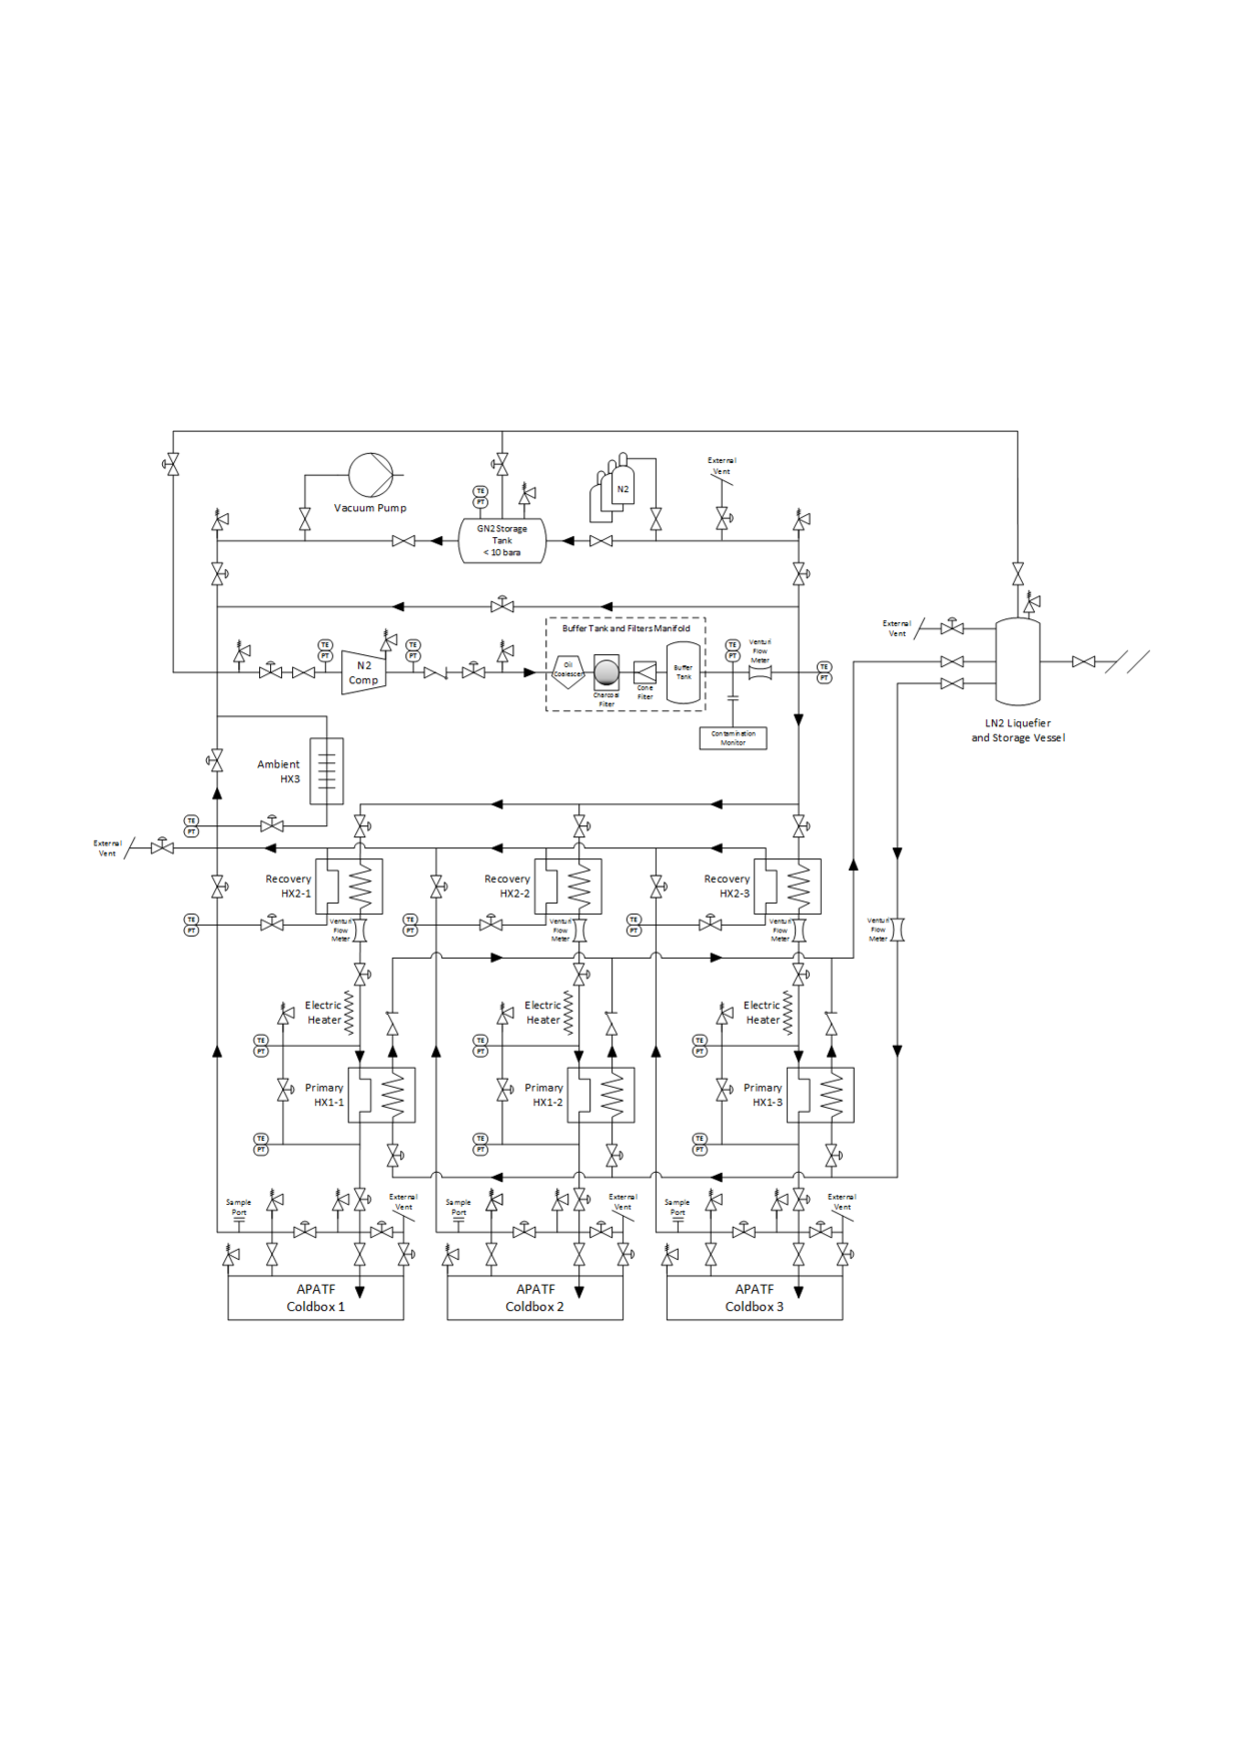
\includegraphics[width=.98\textwidth]{graphics/Cryo-cold-box-mechanical.pdf}
\end{dunefigure}

\begin{dunefigure}[Coldbox cryogenic support system based on LN2 ]{fig:LN2}
  {Layout of the cryogenics supporting the \dword{apa} test facility with open loop refrigeration.}
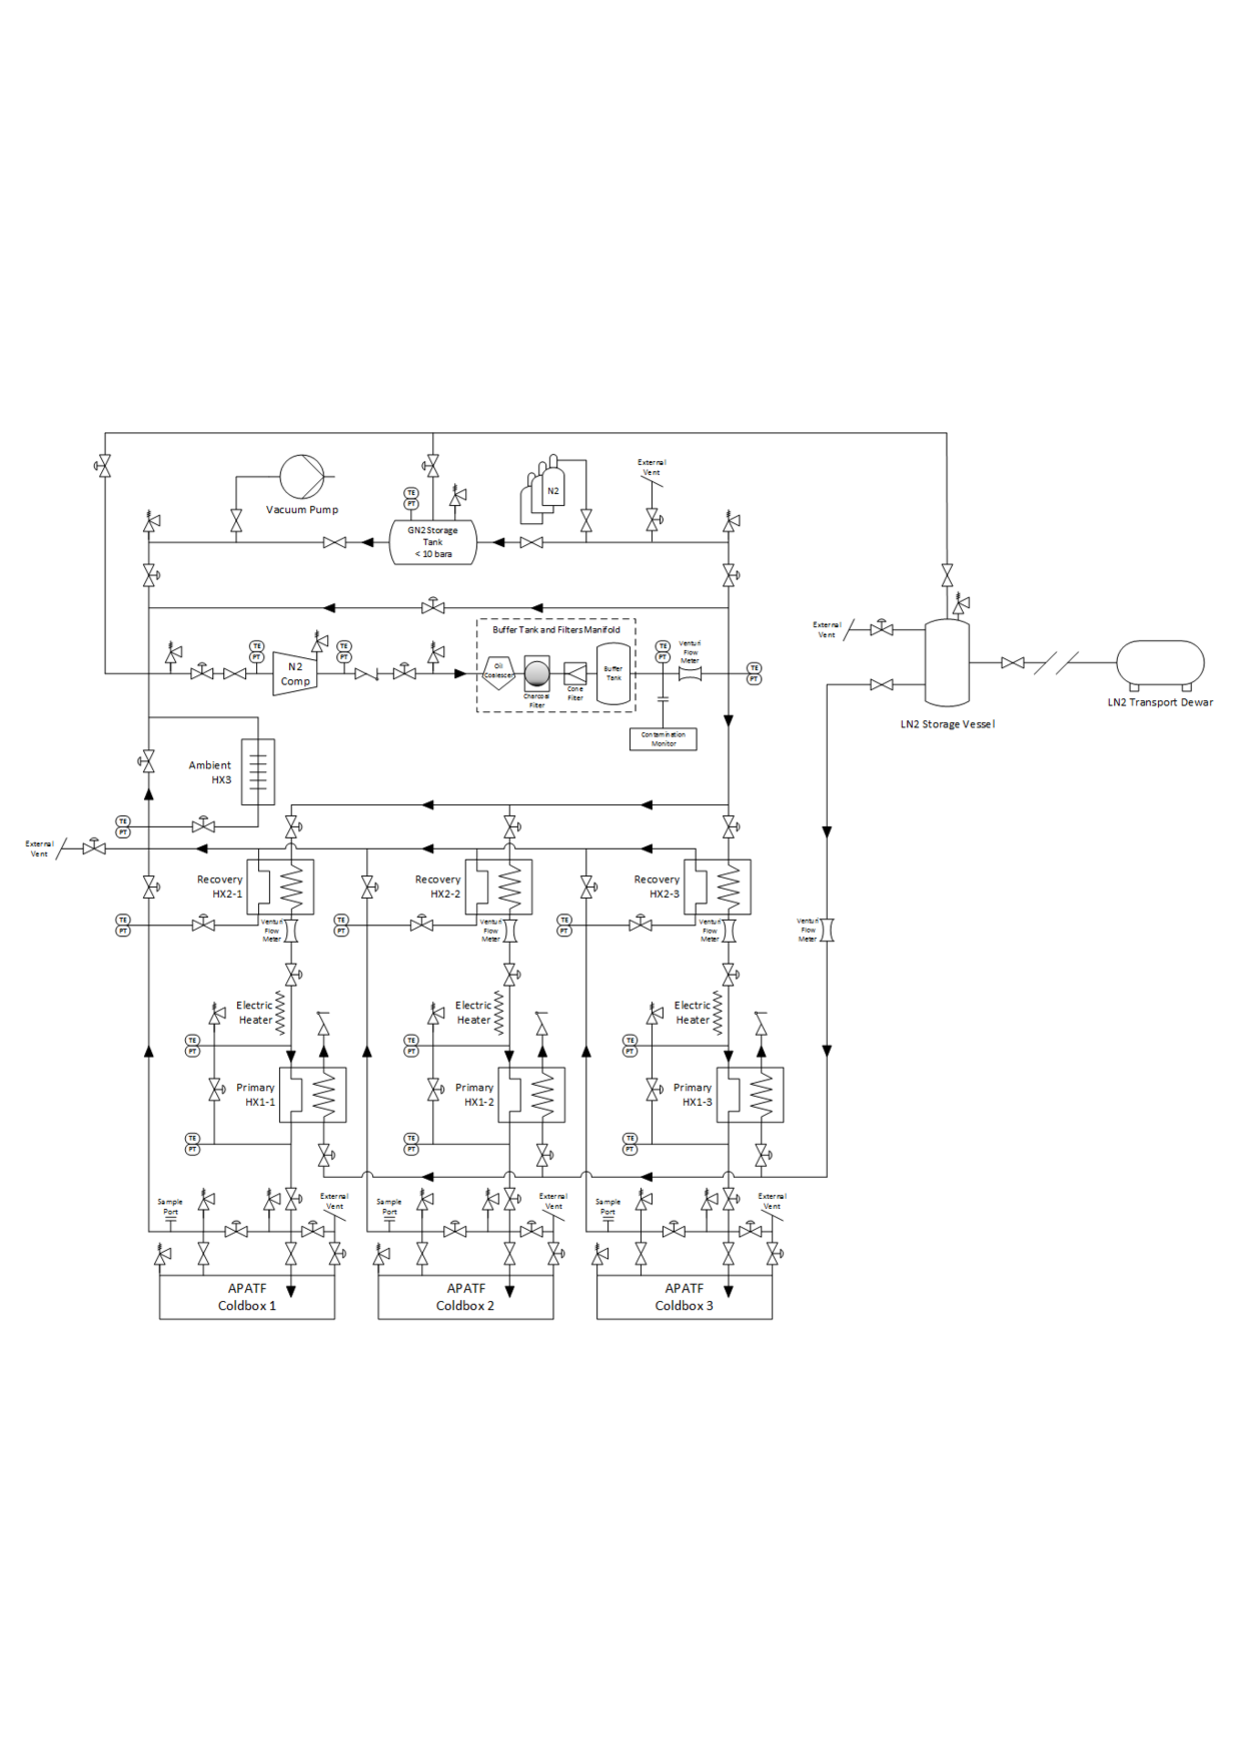
\includegraphics[width=.98\textwidth]{graphics/Cryo-cold-box-LN2.pdf}
\end{dunefigure}



%%%%%%%%%